\documentclass[11pt, oneside]{article}
\usepackage[letterpaper, margin=2cm]{geometry}
\usepackage{booktabs}
\usepackage{Logemann}
\usepackage{Integral}
\usepackage{LinearAlgebra}
\usepackage{Derivative}
\usepackage{Vector}
\usepackage{Sum}
\usepackage{SetTheory}
\usepackage[backend=biber]{biblatex}
\addbibresource{refs.bib}

\title{Discontinuous Galerkin Method for Solving Thin Film Equations}
\author{Caleb Logemann}

\date{December 13, 2018} % Date, can be changed to a custom date

\begin{document}
\maketitle

\begin{abstract}
  This paper will describe a discontinuous Galerkin method for solving
  thin film equations. The model equation is
  $q_t + \p{q^2 - q^3}_x = -\p{q^3 q_{xxx}}_x$.
  This equation will be handled using operator splitting.
  An explicit Runge Kutta discontinuous Galerkin method will be used to solve the
  convection term.
  An implicit local discontinuous Galerkin method will solve the fourth order
  diffusion equation.
  Furthermore a preconditioned linear solver for the implicit method will be
  described.
\end{abstract}

\section{Introduction}
  Thin film equations arise in several applications involving lubrication theory.
  For example thin films of water flowing over an airplane wing during flight.
  When an airplane flies in wet conditions ice can begin to build up on the
  surface of the plane.
  An important part of modeling the accretion of ice on a plane is to study how
  the water might move over the surface of the plane before freezing.
  This is known as runback.
  Thin film equations also arrive in different industrial applications, such as
  industrial coating.

  In these contexts several forces drive the motion of the fluid, including
  gravity, wind shear, and surface tension.
  Beginning with the Navier-Stokes equations shown below,
  \begin{align*}
    \nabla \cdot \v{u} &= 0 \\
    \partial_t \v{u} + \nabla \cdot \p{\v{u}\v{u}} &= - \frac{1}{\rho} \nabla p + \frac{1}{\rho}\nabla \cdot \sigma + \v{g} \\
    \partial_t h_s + \p{u, v}^T \cdot \nabla h_s &= w \\
    \partial_t h_b + \p{u, v}^T \cdot \nabla h_b &= w
  \end{align*}
  and using a lubrication approximation to model these driving forces the model
  equation
  \[
    q_t + \p{q^2 - q^3}_x = -\p{q^3 q_{xxx}}_x
  \]
  can be derived.
  The flux terms $q^2$ and $q^3$ come from the force of gravity and the wind
  shear, and the fourth order diffusion models the surface tension.
  See the review by Myers\cite{myersReview} for a derivation.

\section{Method}
  The model equation will be solved using operator splitting, the convection
  equation
  \[
    q_t + \p{q^2 - q^3}_x = 0
  \]
  and the diffusion equation
  \[
    q_t + \p{q^3 q_{xxx}}_x = 0
  \]
  will be solved consecutively using different methods in order to
  approximate the solution to the original equation.
  In order to achieve 2nd order accuracy Strang splitting can be used.
  In Strang splitting one whole time step, $\Delta t$ consists of stepping the
  convection equation $\frac{1}{2}\Delta t$, the diffusion equation $\Delta t$,
  and the convection equation again by $\frac{1}{2}\Delta t$.

  The discontinuous Galerkin method will be used to solve both of these
  equations, so first some notation will be introduced.
  The domain of this problem $\Omega$ will be some interval on the real line,
  $\br{a, b}$.
  Let this domain be partitioned by $N+1$ evenly spaced points
  $a = x_{1/2} < x_{3/2} < \cdots < x_{i+1/2} < \cdots < x_{N+1/2} = b$.
  Let $h = x_{i+1/2} - x_{i-1/2}$ be the distance between points and let
  $x_i = \frac{1}{2}\p{x_{i-1/2} + x_{i+1/2}}$ be cell centers.
  This partition will create $N$ intervals denoted
  $I_j = \br{x_{j-1/2}, x_{j+1/2}}$.
  The DG space can then be defined as
  $V_h = \set{v \in L^2(\Omega): \eval{v}{I_j} \in P_k(I_j)}$, where $P_k(I_j)$
  is the set of all  polynomials of order $k$ or less.
  In this case the spatial order of the DG method will be $k+1$.
  On a single interval the canonical variable $\xi$ may be used, such that for
  $x \in I_j$, then $\xi \in \br{-1, 1}$.
  This transformation can be defined as $x = x_j + \frac{1}{2}h\xi$.
  When using this variable the model equations become
  \[
    q_t + \frac{2}{\Delta x} \p{q^2 - q^3}_\xi = 0
  \]
  and
  \[
    q_t + \frac{16}{\Delta x^4} \p{q^3 q_{xxx}}_x = 0
  \]

\subsection{Convection Equation}
  The convection equation will be handled using the standard Runge Kutta
  discontinuous Galerkin method.
  This method can be described as finding a function $Q(t, x)$ such that for
  every $t > 0$, $Q(t, \cdot) \in V_h$ and that satisfies
  \begin{align*}
    \dintt{I_j}{}{Q_t v}{x} &= \dintt{I_j}{}{f(Q)v_x}{x} - \p{\mcF_{j + 1/2}v^-(x_{j+1/2}) - \mcF_{j - 1/2}v^+(x_{j-1/2})}
  \end{align*}
  for all $v \in V_h$, where the numerical flux is the local Lax-Friedrichs flux
  given by
  \[
    \mcF_{j+1/2} = \frac{1}{2}\p{f\p{Q^-_{j+1/2}} + f\p{Q^+_{j+1/2}}} + \max[q]{\abs{f'(q)}}\p{Q^-_{j+1/2} - Q^+_{j+1/2}}.
  \]
  If the Legendre polynomials, $\phi^{\ell}$ are used as a basis for the DG space on each
  element, then the semi-discrete form of this method is
  \[
    \dot{Q_i^{\ell}} = \frac{1}{\Delta x}\dintt{-1}{1}{f(Q_i)\phi_{\xi}^{\ell}}{\xi} - \frac{1}{\Delta x} \p{\mcF_{i + 1/2}\phi(1) - \mcF_{i - 1/2}\phi(-1)}
  \]
  where
  \[
    \mcF_{j+1/2} = \frac{1}{2}\p{f\p{Q_{i+1}(-1)} + f\p{Q_{i}(1)}} + \max[q]{\abs{f'(q)}}\p{Q_{i}(1) - Q_{i+1}(-1)}.
  \]

  This system of ordinary differential equations can now be solved using any ODE
  solver.
  I will denote this system at
  \[
    \dot{\v{Q}} = L(\v{Q}).
  \]
  For a first order solver, the forward Euler method will be used
  \[
    \v{Q}^{n+1} = \v{Q}^n + L(\v{Q}^n)
  \]
  and for a second order solver the following Runge Kutta method will
  be used
  \begin{align*}
    \v{Q}^{\star} &= \v{Q}^n + \Delta t L(\v{Q}^n) \\
    \v{Q}^{n+1} &= \frac{1}{2}\p{\v{Q}^n + \v{Q}^{\star}} + \frac{1}{2} \Delta t L(\v{Q}^{\star}).
  \end{align*}
  Both of these time stepping methods are strong stability preserving (SSP),
  that is they are total variation diminishing.
  Also note that a CFL condition on the size of the time step is necessary for
  this stability.
  The time step will need to be on the same order as the order of $h$, that is
  $O(\Delta t) = O(h)$.
  This means that as $h$ is refined the size of the time step will need to be
  refined as well.
  However this condition is standard and not too onerous.

\subsection{Diffusion Equation}
  The local discontinuous Galerkin (LDG) method will be used to solve the fourth order
  diffusion equation.
  This method was first developed by Cockburn and Shu in 1998 \cite{cockburn1998local}.
  The fourth order diffusion equation
  \begin{align*}
    q_t + \p{q^3 q_{xxx}}_x &= 0
  \end{align*}
  will be rewritten in the following form by introducing auxilliary variables
  \begin{align*}
    r &= q_{x} \\
    s &= r_{x} \\
    u &= q^3 s_{x} \\
    q_t &= -u_{x}.
  \end{align*}
  In order to linearize this system, let $\eta = \p{Q^n}^3$, that is use the
  value of $Q$ at the previous time step as a constant function.
  This will allow the a linear system of ODEs to be formed instead of being
  nonlinear in $Q$.
  The LDG method can then be described as finding $Q(t, \cdot), R, S, U \in V_h$
  such that
  \begin{align*}
    \dintt{I_j}{}{R v}{x} &= -\dintt{I_j}{}{Q v_x}{x} + \p{\hat{Q}_{j+1/2}v^-_{j+1/2} - \hat{Q}_{j-1/2} v^+_{j-1/2}} \\
    \dintt{I_j}{}{S w}{x} &= -\dintt{I_j}{}{R w_x}{x} + \p{\hat{R}_{j+1/2}w^-_{j+1/2} - \hat{R}_{j-1/2} w^+_{j-1/2}} \\
    \dintt{I_j}{}{U y}{x} &= \dintt{I_j}{}{S_x \eta y}{x} - \p{S^-_{j+1/2}\eta^-_{j+1/2}y^-_{j+1/2} - S^+_{j-1/2}\eta^+_{j-1/2}y^+_{j-1/2}} \\
    &+ \p{\hat{S}_{j+1/2} \hat{\eta}_{j+1/2} y^-_{j+1/2} - \hat{S}_{j-1/2} \hat{\eta}_{j-1/2} y^+_{j-1/2}} \\
    \dintt{I_j}{}{Q_t z}{x} &= -\dintt{I_j}{}{U z_x}{x} + \p{\hat{U}_{j+1/2}z^-_{j+1/2} - \hat{U}_{j-1/2} z^+_{j-1/2}}
  \end{align*}
  for all $I_j \in \Omega$ and all $v, w, y, z \in V_h$.
  In this case the numerical fluxes are the so called alternating fluxes and the
  $\eta$ flux is just an average flux.
  \begin{align*}
    \hat{\eta}_{j+1/2} &= \frac{1}{2}\p{\eta^+_{j+1/2} + \eta^-_{j+1/2}} \\
    \hat{Q}_{j+1/2} &= Q^+_{j+1/2} \\
    \hat{R}_{j+1/2} &= R^-_{j+1/2} \\
    \hat{S}_{j+1/2} &= S^+_{j+1/2} \\
    \hat{U}_{j+1/2} &= U^-_{j+1/2}
  \end{align*}
  The alternating fluxes just evaluate the flux on one side of the interface
  and alternate sides with the order of derivative.

  This method result in a system of ODEs, much in the same way that the
  Runge Kutta discontinuous Galerkin method does.
  However if this system was to be solved explicitly as the RKDG method is,
  there would be a severe time step restriction.
  The time step would need to scale with the $h^4$.
  This is quite restrictive, and as $h$ was refined the time step would quickly
  become impossibly small.
  Therefore this system needs to be solved implicitly so that the method is
  stable with much larger time steps.
  The first order method used is the backward Euler method.
  \begin{align*}
    \v{Q}^{n+1} = \v{Q}^n + \Delta t L(\v{Q}^{n+1})
  \end{align*}
  The second order method used is
  \begin{align*}
    \v{Q}^{\star} &= \v{Q}^n + \frac{1}{4} \Delta t \p{L(\v{Q}^n) + L(\v{Q}^{\star})} \\
    3 q^{n+1} &= 4 \v{Q}^{\star} - \v{Q}^{n} + \Delta t L(\v{Q}^{n+1})
  \end{align*}
  Both of these methods work well with the same time step restriction as for the
  RKDG method for the convection equation.

  These implicit method require solving a linear system.
  The Generalized Minimal Residual (GMRES) method was used to solve the
  necessary linear systems.
  The GMRES method is an iterative linear solver that solves a linear system by
  minimizing the residual, $\v{r} = A\v{x} - \v{b}$ over the space
  $K_n = \spanspace{\v{b}, A\v{b}, A^2\v{b}, \cdots, A^{n-1}\v{b}}$.
  Unfortunately the linear systems generated by these methods are rather
  ill-conditioned.
  This means that as $h$ is refined and the size of the system increases the
  number of iterations required for the GMRES method to converge scales with
  the size of the system.
  This means that as $h$ is refined the time that it take to solve the linear
  system will grow dramatically.
  In order to accelerate convergence a preconditioner is used.
  The linear system evolves over time because the linear system depends on
  $Q$.
  Picking a value for $Q$ and then computing the exact inverse of the linear
  system could be a good preconditioner as long as the solution stays near the
  chosen value of $Q$.
  In this case the initial condition was chosen for the value of $Q$, that is at
  the beginning of the simulation the inverse of the linear system is found and
  then used as the preconditioner for the remainder of the simulation.
  We let $P = A_0^{-1}$ and then solve the preconditioned system
  $PA\v{x} = P\v{b}$ instead.
  This is believed to significanly accelerate the convergence, but it has yet to
  be shown.

\section{Results}
  Both the Runge Kutta discontinuous Galerkin and the local discontinuous
  Galerkin along with the operator splitting were implemented as part of
  the {\sc{DoGPack}} software package\cite{dogpack}.
  Two examples will be presented.
  The first example will be a Riemann problem.
  The left state of the riemann problem is $q = 0.3323$ and the right state is
  $q = 0.1$.
  The domain is $x \in \br{0, 40}$ with the discontinuity at $x = 5.0$.
  This example is run to time $T = 60$, with CFL condition number of $0.2$.
  This example shows how wave propogating to the right can extend above and
  below the left and right states at the shock location.
  This is also the behavior shown by Youngsoo Ha et. al in \cite{ha2008numerical}.
  \begin{center}
    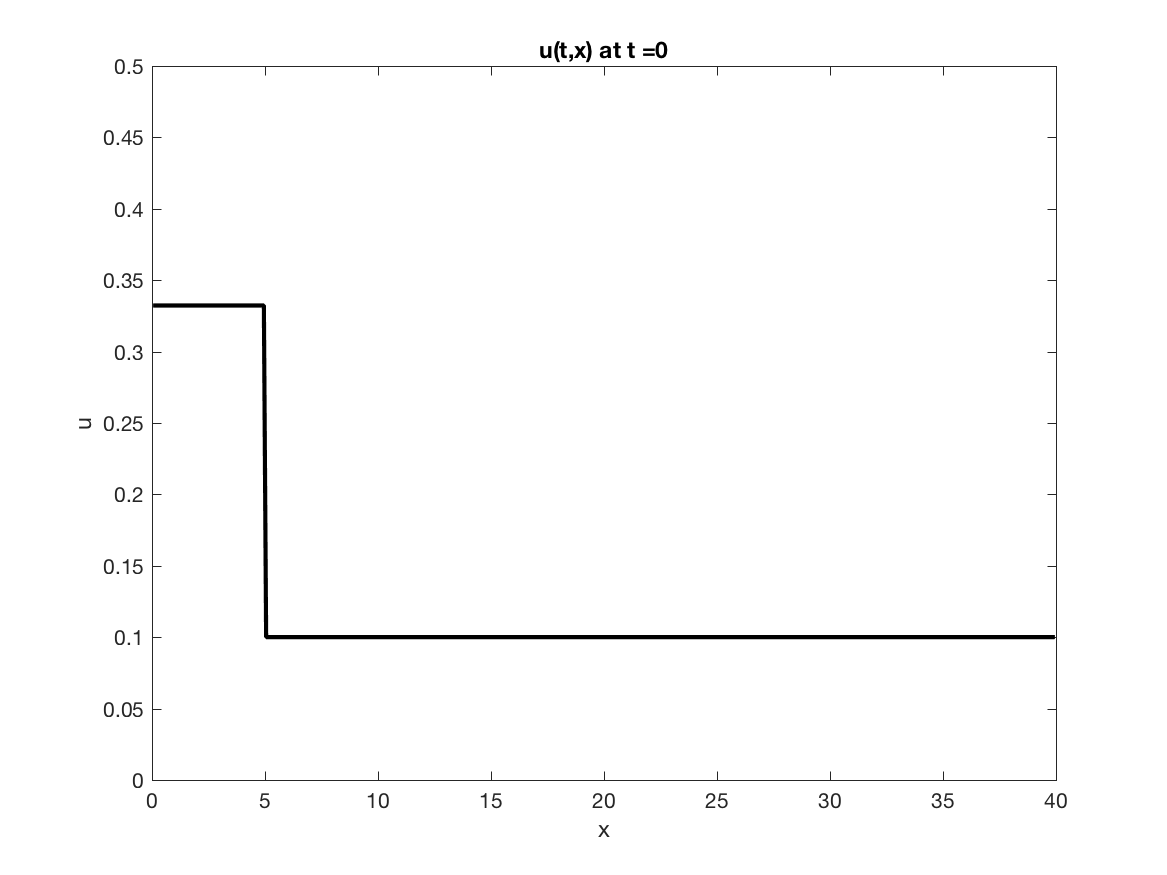
\includegraphics[scale=0.4]{Figures/reimann0.png}
    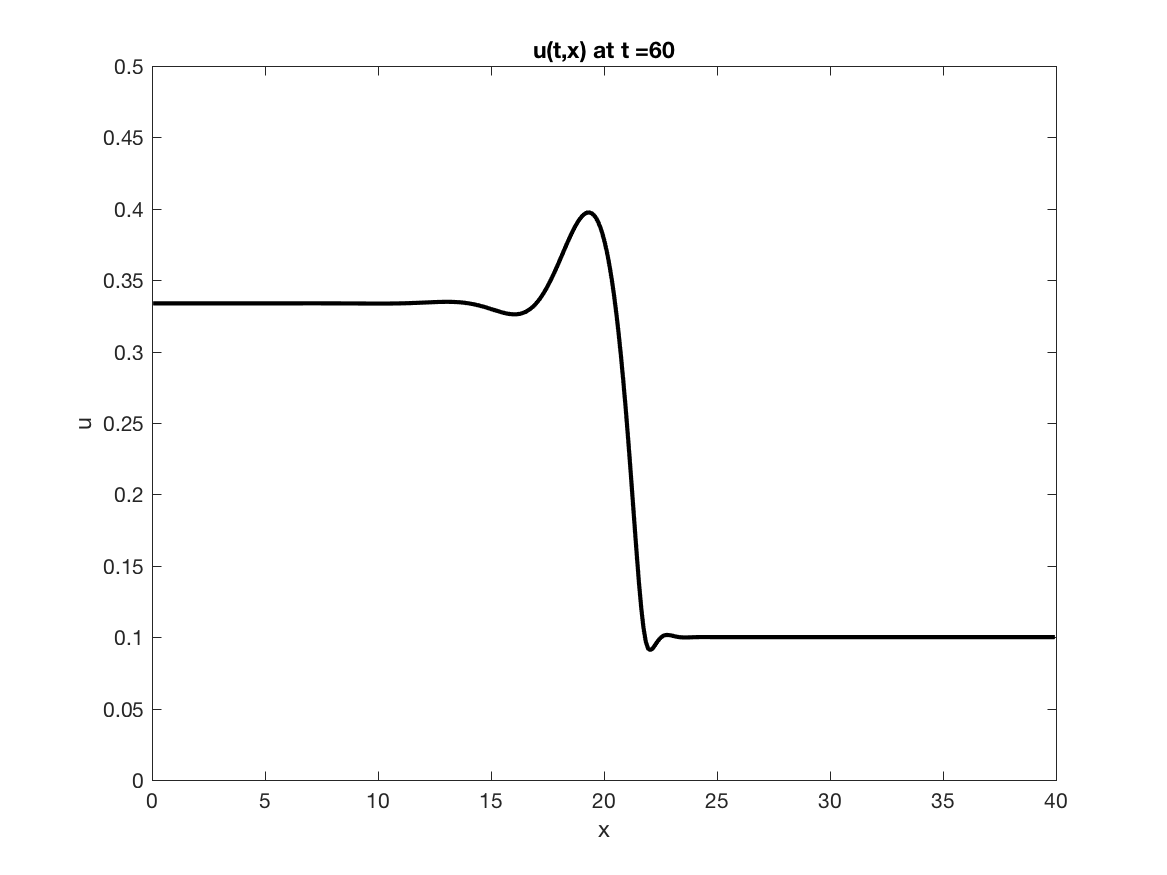
\includegraphics[scale=0.4]{Figures/reimann60.png}
  \end{center}

  The second example will be of a square wave.
  The domain for this problem is $x \in \br{-1.5, 6.5}$, with $h = 0.04$.
  The initial condition is $q = 0.6666$ in $x \in \br{0, 1}$ and $q = 0$
  otherwise.
  This is simulated to $T = 20$ with a CFL number of $0.2$.
  The surface tension quickly rounds out the profile, and the wind shear
  stretches out the fluid.
  \begin{center}
    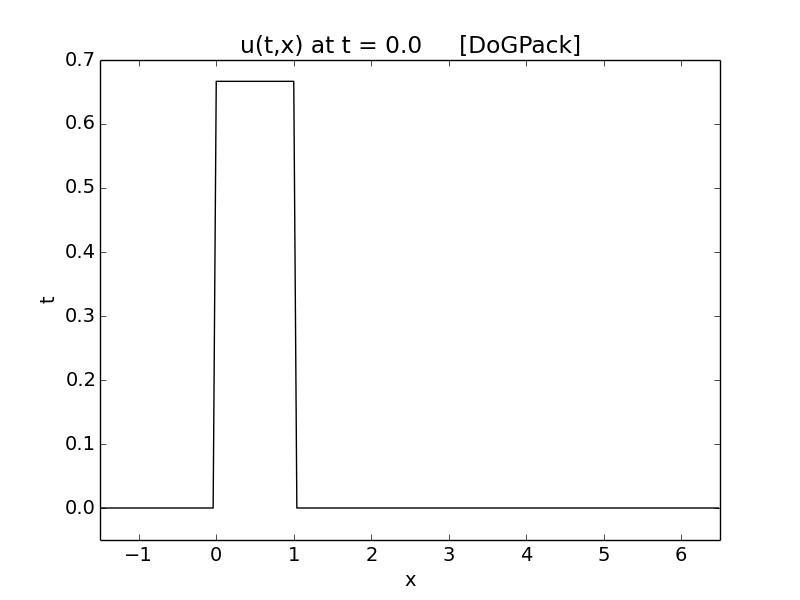
\includegraphics[scale=0.4]{Figures/squareWaveInitial.png}
    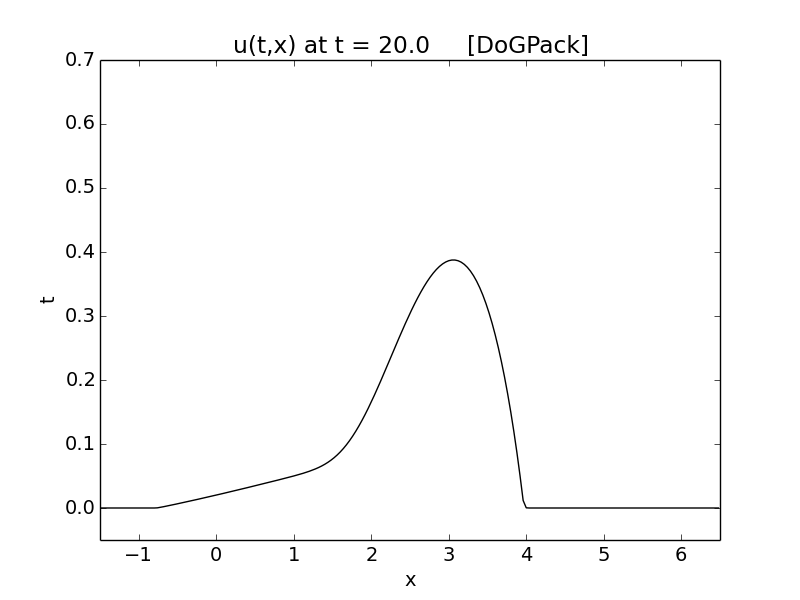
\includegraphics[scale=0.4]{Figures/squareWaveFinal.png}
  \end{center}

\section{Conclusion}
  This paper has described a discontinuous Galerkin method for solving the
  thin film equation
  \[
    q_t + \p{q^2 - q^3}_x = \p{q^3 q_{xxx}}_x
  \]
  using operator splitting, RKDG, and LDG.
  Preconditioned GMRES is used to solve the linear system from the implicit
  time stepping.
  This method should be able to attain second order accuracy.
  There is still some work to be done on this problem.
  The second order accuracy needs to be formally shown using a manufactured
  solution.
  Also the efficacy of the preconditioner needs to be analyzed.

  \printbibliography{}

\end{document}
